\begin{frame}
	\framesubtitle{Подтверждение ММЧВС}
	\frametitle{Измерение спектра при известном модовом составе}
	
	
	\begin{columns}
		\begin{column}{0.5\textwidth}
			\centering
			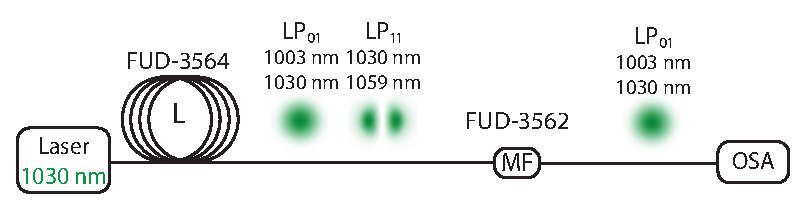
\includegraphics[width=\linewidth]{Dissertation/images/imfwm/scheme_osa.eps}
			
			\footnotesize{Блок-схема экспериментальной установки для определения спектрального состава излучения в поперечной моде $\LPii$.\\MF: модовый фильтр;\\OSA: анализатор спектра.}
		\end{column}
		
		\begin{column}{0.5\textwidth}
			\centering
			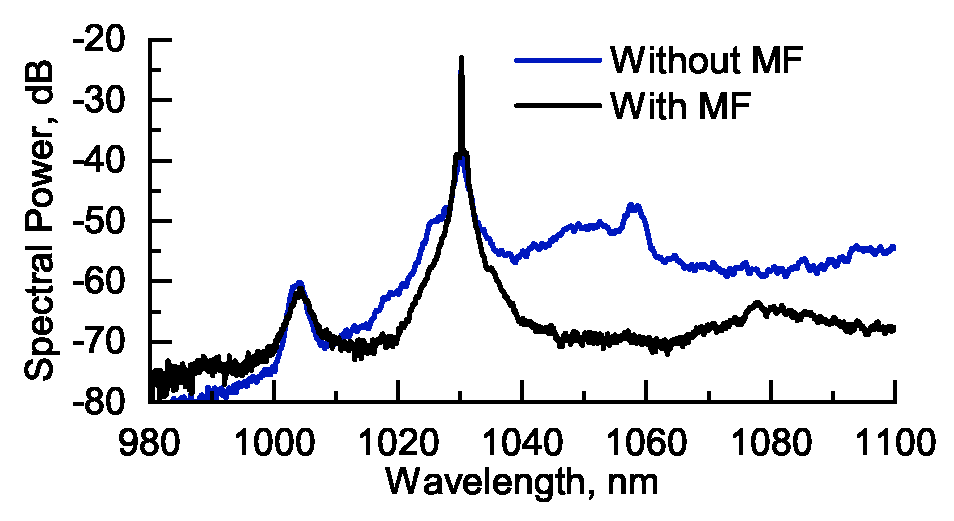
\includegraphics[width=\linewidth]{Dissertation/images/imfwm/mode_filter_spectra}
			
			\footnotesize{Спектры в области $1~\text{мкм}$ с применением (чёрный) и без применения (синий) МФ.}
		\end{column}
	\end{columns}

	
	
%	На рис. синяя и чёрная кривые соответствуют спектрам с модовым фильтром (МФ) и без него соответственно. МФ~--- это участок одномодового ОВ FUD-3562, согласованного по модовому диаметру с ОВ доставки. В спектральных областях $1030~\text{нм}$ (накачка) и $1003~\text{нм}$ (антистоксовая компонента) различия между спектрами минимальны, что указывает на сохранение этих компонент при распространении излучения через МФ. В спектральной области около $1059~\text{нм}$ (стоксовая компонента) МФ ослабляет излучение на $20~\text{дБ}$, что свидетельствует о присутствии моды $\LPii$ в данной спектральной области.
	
\end{frame}

\begin{frame}
	\framesubtitle{Подтверждение ММЧВС}
	\frametitle{Определение модового состава при известном спектре}

	\centering
	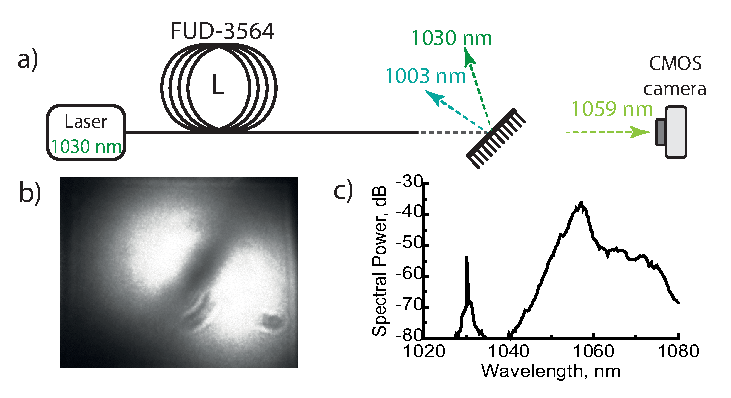
\includegraphics[width=0.7\linewidth]{Dissertation/images/imfwm/scheme_mirror.eps}
	
	\footnotesize{a) Экспериментальная установка для визуализации пучка на длине волны $1059$~нм;\\b) изображение пучка на длине волны $1059$~нм\\ c) спектр после дихроичного зеркала.}

	


\end{frame}

\begin{frame}
	\framesubtitle{Взаимное влияние процессов четырёхволнового смешения в оптических волокнах}
	\frametitle{Математическая модель ЧВС}
	Связанные уравнения для амплитуд\footnote{Agrawal, G. P. Nonlinear Fiber Optics. 6th ed. London ; San Diego, CA : Academic Press, 2019. Eqs. (10.2.2)–(10.2.5).}:
	\begin{columns}
		\begin{column}{0.48\textwidth}
			\scalebox{0.72}{%
				\begin{minipage}{\textwidth}
					\begin{equation*}
						\left\{\begin{array}{@{}l@{}}
							\dfrac{dA_1}{dz}=\dfrac{\im n_{nl} \omega_1}{c}\!\left[\left(f_{11}\left|A_1\right|^2+\sum\limits_{k\neq1}f_{1k}\left|A_k\right|^2\right)\!A_1+2f_{1234}A_2^{\ast}A_3A_4\e^{\im \Delta k z}\right]\!, \vspace{0.05cm} \\ 
							\dfrac{dA_2}{dz}=\dfrac{\im n_{nl} \omega_2}{c}\!\left[\left(f_{22}\left|A_2\right|^2+\sum\limits_{k\neq2}f_{2k}\left|A_k\right|^2\right)\!A_2+2f_{2134}A_1^{\ast}A_3A_4\e^{\im \Delta k z}\right], \vspace{0.05cm} \\
							\dfrac{dA_3}{dz}=\dfrac{\im n_{nl} \omega_3}{c}\!\left[\left(f_{33}\left|A_3\right|^2+\sum\limits_{k\neq3}f_{3k}\left|A_k\right|^2\right)\!A_3+2f_{3412}A_4^{\ast}A_2A_1\e^{-\im \Delta k z}\right], \vspace{0.05cm} \\
							\dfrac{dA_4}{dz}=\dfrac{\im n_{nl} \omega_4}{c}\!\left[\left(f_{44}\left|A_4\right|^2+\sum\limits_{k\neq4}f_{4k}\left|A_k\right|^2\right)\!A_4+2f_{4312}A_3^{\ast}A_2A_1\e^{-\im \Delta k z}\right].
						\end{array}\right.\,	
					\end{equation*}
				\end{minipage}
			}
		\end{column}
		\begin{column}{0.52\textwidth}
			$A_{{i}}$~--- амплитуды взаимодействующих волн с циклическими частотами $\omega_i$;
			
			$n_{nl}$~--- нелинейный показатель преломления;
			
			$f_{ij}\text{ и }f_{ijkl}, i,j,k,l = \overline{1,4}$ ~--- интегралы перекрытия между поперечными модами ОВ и их парами соответственно;
			
							$z$~--- продольная координата;
			
			$\Delta k$~--- волновая расстройка;
			
			${n_{i}}$~--- эффективный модовый показатель преломления;
			
			$c$~--- скорость света в вакууме
		\end{column}
	\end{columns}
	
	\vfill

\end{frame}


\begin{frame}
	\frametitle{Модель экситонов с переносом заряда}
	\framesubtitle{Кривые фазового синхронизма при ГВГ в оптических волокнах}
	
	Модель экситонов с переносом заряда (ЭПЗ)\footnote{\scriptsize Антонюк Б. П., Антонюк В. Б. Самоорганизация возбуждений в германосиликатных волоконных световодах и ее роль в генерации второй гармоники //Успехи физических наук. – 2001. – Т. 171. – №. 1. – С. 61-78.}:
	
	\begin{itemize}
		\item Возбуждение \textbf{одним} квантом зелёного света, переход электрона с примесного Ge-центра в матрицу или на другой Ge-центр.
		\item \textbf{Самоорганизация} ЭПЗ: в слабом затравочном электрическом поле образуется положительная обратная связь --- диполи ориентируются преимущественно против поля.
	\end{itemize}
	
	\centering
	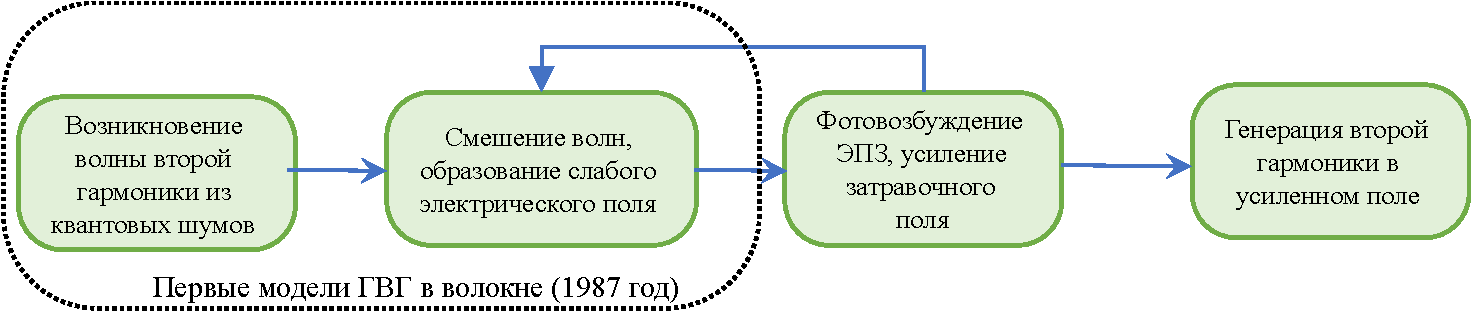
\includegraphics[width=0.9\linewidth]{Presentation/images/scheme_epz}

\end{frame}

%\begin{frame}
%    \frametitle{Ответы на замечания ведущей организации НИИ~<<Рога~и~копыта>>}
%    \begin{itemize}
%        \item Замечание -- ответ
%        \item Замечание -- ответ
%        \item Замечание -- ответ
%        \item Замечание -- ответ
%        \item Замечание -- ответ
%    \end{itemize}
%\end{frame}
%
%\begin{frame}
%    \frametitle{Ответы на замечания оф. оппонента Иванова\,И.\,И}
%    \begin{itemize}
%        \item Замечание -- ответ
%        \item Замечание -- ответ
%        \item Замечание -- ответ
%        \item Замечание -- ответ
%        \item Замечание -- ответ
%    \end{itemize}
%\end{frame}
%
%\begin{frame}
%    \frametitle{Ответы на замечания Петрова\,П.\,П}
%    \begin{itemize}
%        \item Замечание -- ответ
%        \item Замечание -- ответ
%        \item Замечание -- ответ
%        \item Замечание -- ответ
%        \item Замечание -- ответ
%    \end{itemize}
%\end{frame}
